\definecolor{azul}{RGB}{0,0,191}
\begin{minipage}{1\textwidth}
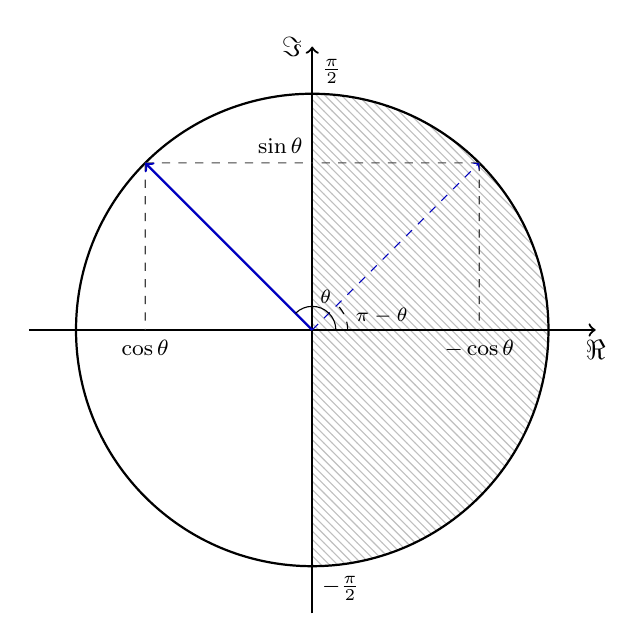
\begin{tikzpicture}[scale=3]
    \usetikzlibrary{patterns}

    % Preenchimento do lado direito do círculo
    \fill[pattern=north west lines, pattern color=lightgray] (0,0) -- (90:1) arc (90:-90:1) -- cycle;

    % Eixos coordenados
    \draw[->, thick] (-1.2,0) -- (1.2,0) node[below] {$\Re$};
    \draw[->, thick] (0,-1.2) -- (0,1.2) node[left] {$\Im$};
    
    % Círculo unitário
    \draw[thick] (0,0) circle (1);
    
    % Ângulo genérico
    \def\ang{45} % Pode alterar este valor
    \coordinate (O) at (0,0);
    \coordinate (M) at (0,-1);
    \coordinate (B) at (0, 1);
    \coordinate (P) at ({\ang}:1);
    \coordinate (P2) at ({180-\ang}:1);
    
    % Projeções
    \draw[dashed, darkgray] (P) -- ({cos(\ang)},0) node[black,below] {\footnotesize$-\cos \theta$};
    \draw[dashed, darkgray] (P) -- (0,{sin(\ang)}) node[black,above left] {\footnotesize$\sin \theta$};
    \draw[dashed, darkgray] (P2) -- ({-cos(\ang)},0) node[black,below] {\footnotesize$\cos \theta$};
    \draw[dashed, darkgray] (P2) -- (0,{sin(\ang)});
    
    % Raio
    \draw[->, dashed, azul] (O) -- (P);
    \draw[->, thick, azul] (O) -- (P2);
    
    % Ângulo
    \draw (0.1,0) arc (0:{180-\ang}:0.1);
    \node at ({0.5*(180-\ang)}:0.15) {\scriptsize$\theta$};
    \draw[dashed] (0.15,0) arc (0:{\ang}:0.15);
    \node at ({0.25*\ang}:0.3) {\scriptsize$\pi - \theta$};

    \node[below right] at (M) {\footnotesize$-\frac{\pi}{2}$};
    \node[above right] at (B) {\footnotesize$\frac{\pi}{2}$};

\end{tikzpicture}
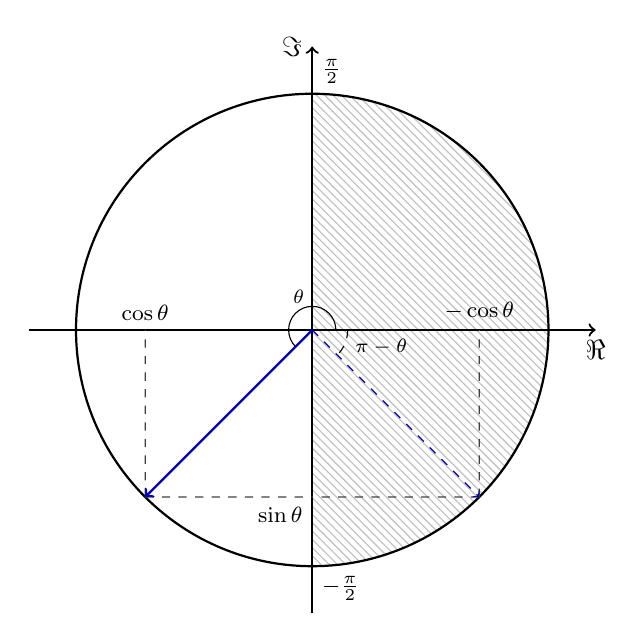
\begin{tikzpicture}[scale=3]
    \usetikzlibrary{patterns}

    % Preenchimento do lado direito do círculo
    \fill[pattern=north west lines, pattern color=lightgray] (0,0) -- (90:1) arc (90:-90:1) -- cycle;

    % Eixos coordenados
    \draw[->, thick] (-1.2,0) -- (1.2,0) node[below] {$\Re$};
    \draw[->, thick] (0,-1.2) -- (0,1.2) node[left] {$\Im$};
    
    % Círculo unitário
    \draw[thick] (0,0) circle (1);
    
    % Ângulo genérico
    \def\ang{45} % Pode alterar este valor
    \coordinate (O) at (0,0);
    \coordinate (M) at (0,-1);
    \coordinate (B) at (0, 1);
    \coordinate (P) at ({-\ang}:1);
    \coordinate (P2) at ({180+\ang}:1);
    
    % Projeções
    \draw[dashed, darkgray] (P) -- ({cos(\ang)},0) node[black,above] {\footnotesize$-\cos \theta$};
    \draw[dashed, darkgray] (P) -- (0,{-sin(\ang)}) node[black,below left] {\footnotesize$\sin \theta$};
    \draw[dashed, darkgray] (P2) -- ({-cos(\ang)},0) node[black,above] {\footnotesize$\cos \theta$};
    \draw[dashed, darkgray] (P2) -- (0,{-sin(\ang)});
    
    % Raio
    \draw[->, dashed, azul] (O) -- (P);
    \draw[->, thick, azul] (O) -- (P2);
    
    % Ângulo
    \draw (0.1,0) arc (0:{180+\ang}:0.1);
    \node at ({0.5*(180+\ang)}:0.15) {\scriptsize$\theta$};
    \draw[dashed] (0.15,0) arc (0:{-\ang}:0.15);
    \node at ({0.3*(-\ang)}:0.3) {\scriptsize$\pi - \theta$};

    \node[below right] at (M) {\footnotesize$-\frac{\pi}{2}$};
    \node[above right] at (B) {\footnotesize$\frac{\pi}{2}$};

\end{tikzpicture}
\end{minipage}
\begin{minipage}{1\textwidth}
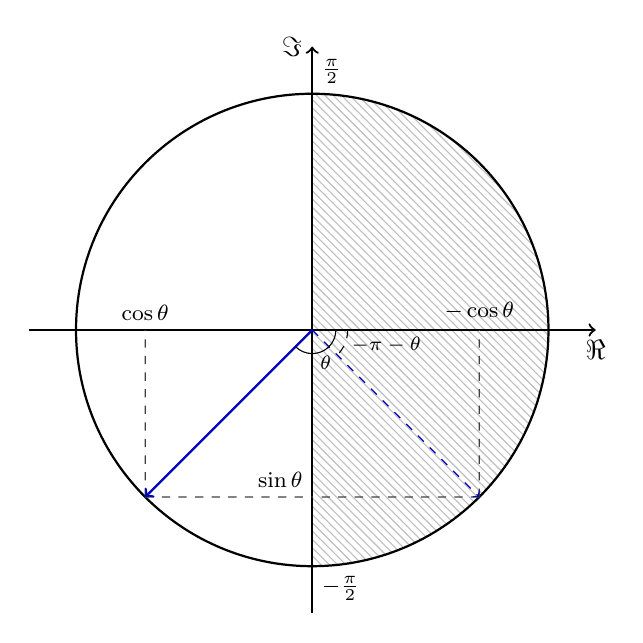
\begin{tikzpicture}[scale=3]
    \usetikzlibrary{patterns}

    % Preenchimento do lado direito do círculo
    \fill[pattern=north west lines, pattern color=lightgray] (0,0) -- (90:1) arc (90:-90:1) -- cycle;

    % Eixos coordenados
    \draw[->, thick] (-1.2,0) -- (1.2,0) node[below] {$\Re$};
    \draw[->, thick] (0,-1.2) -- (0,1.2) node[left] {$\Im$};
    
    % Círculo unitário
    \draw[thick] (0,0) circle (1);
    
    % Ângulo genérico
    \def\ang{-45} % Pode alterar este valor
    \coordinate (O) at (0,0);
    \coordinate (M) at (0,-1);
    \coordinate (B) at (0, 1);
    \coordinate (P) at ({\ang}:1);
    \coordinate (P2) at ({-180-\ang}:1);
    
    % Projeções
    \draw[dashed, darkgray] (P) -- ({cos(\ang)},0) node[black,above] {\footnotesize$-\cos \theta$};
    \draw[dashed, darkgray] (P) -- (0,{sin(\ang)}) node[black,above left] {\footnotesize$\sin \theta$};
    \draw[dashed, darkgray] (P2) -- ({-cos(\ang)},0) node[black,above] {\footnotesize$\cos \theta$};
    \draw[dashed, darkgray] (P2) -- (0,{sin(\ang)});
    
    % Raio
    \draw[->, dashed, azul] (O) -- (P);
    \draw[->, thick, azul] (O) -- (P2);
    
    % Ângulo
    \draw (0.1,0) arc (0:{-180-\ang}:0.1);
    \node at ({0.5*(-180-\ang)}:0.15) {\scriptsize$\theta$};
    \draw[dashed] (0.15,0) arc (0:{\ang}:0.15);
    \node at ({0.25*\ang}:0.32) {\scriptsize$-\pi - \theta$};

    \node[below right] at (M) {\footnotesize$-\frac{\pi}{2}$};
    \node[above right] at (B) {\footnotesize$\frac{\pi}{2}$};

\end{tikzpicture}
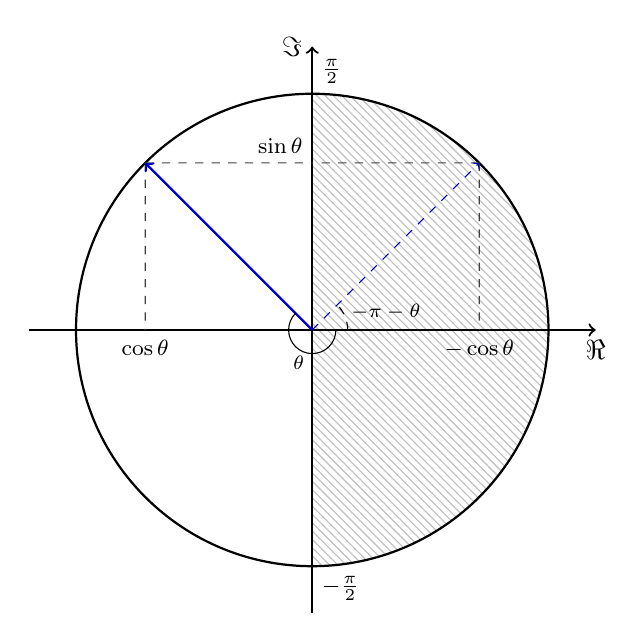
\begin{tikzpicture}[scale=3]
    \usetikzlibrary{patterns}

    % Preenchimento do lado direito do círculo
    \fill[pattern=north west lines, pattern color=lightgray] (0,0) -- (90:1) arc (90:-90:1) -- cycle;

    % Eixos coordenados
    \draw[->, thick] (-1.2,0) -- (1.2,0) node[below] {$\Re$};
    \draw[->, thick] (0,-1.2) -- (0,1.2) node[left] {$\Im$};
    
    % Círculo unitário
    \draw[thick] (0,0) circle (1);
    
    % Ângulo genérico
    \def\ang{-225} % Pode alterar este valor
    \coordinate (O) at (0,0);
    \coordinate (M) at (0,-1);
    \coordinate (B) at (0, 1);
    \coordinate (P) at ({\ang}:1);
    \coordinate (P2) at ({-180-\ang}:1);
    
    % Projeções
    \draw[dashed, darkgray] (P) -- ({cos(\ang)},0) node[black,below] {\footnotesize$\cos \theta$};
    \draw[dashed, darkgray] (P) -- (0,{sin(\ang)}) node[black,above left] {\footnotesize$\sin \theta$};
    \draw[dashed, darkgray] (P2) -- ({-cos(\ang)},0) node[black,below] {\footnotesize$-\cos \theta$};
    \draw[dashed, darkgray] (P2) -- (0,{sin(\ang)});
    
    % Raio
    \draw[->, thick, azul] (O) -- (P);
    \draw[->, dashed, azul] (O) -- (P2);
    
    % Ângulo
    \draw (0.1,0) arc (0:{\ang}:0.1);
    \node at ({0.5*(\ang)}:0.15) {\scriptsize$\theta$};
    \draw[dashed] (0.15,0) arc (0:{-180-\ang}:0.15);
    \node at ({0.3*(-180-\ang)}:0.32) {\scriptsize$-\pi - \theta$};

    \node[below right] at (M) {\footnotesize$-\frac{\pi}{2}$};
    \node[above right] at (B) {\footnotesize$\frac{\pi}{2}$};

\end{tikzpicture}
\end{minipage}